\newpage
\section{Part G}
\label{sec:sec_g}

The same experiment from the previous section was reran, with the modification of targeting the GPU. The hardware being tested on was an \textit{AMD 7900 GRE} using \textit{ROCm} support for \textit{pytorch}.

\LST{part\_g}

Surprisingly, as shown in Figure~\ref{fig:g}, when processing on the GPU the comparable runtimes were actually slower than on the CPU. This result is likely because the dataset is so small that the overhead associated with moving the data to/from the GPU and launching the kernels negates any performance improvements that come from processing on the GPU. Also since the Linear Regression model is only a single (6,1) neuron there isn't mass parallelization available for each parameter like there would be in a deep model. Additionally the ROCm framework is not as well optimized as the CUDA based implementations.

\begin{figure}[htpb]
	\centering
	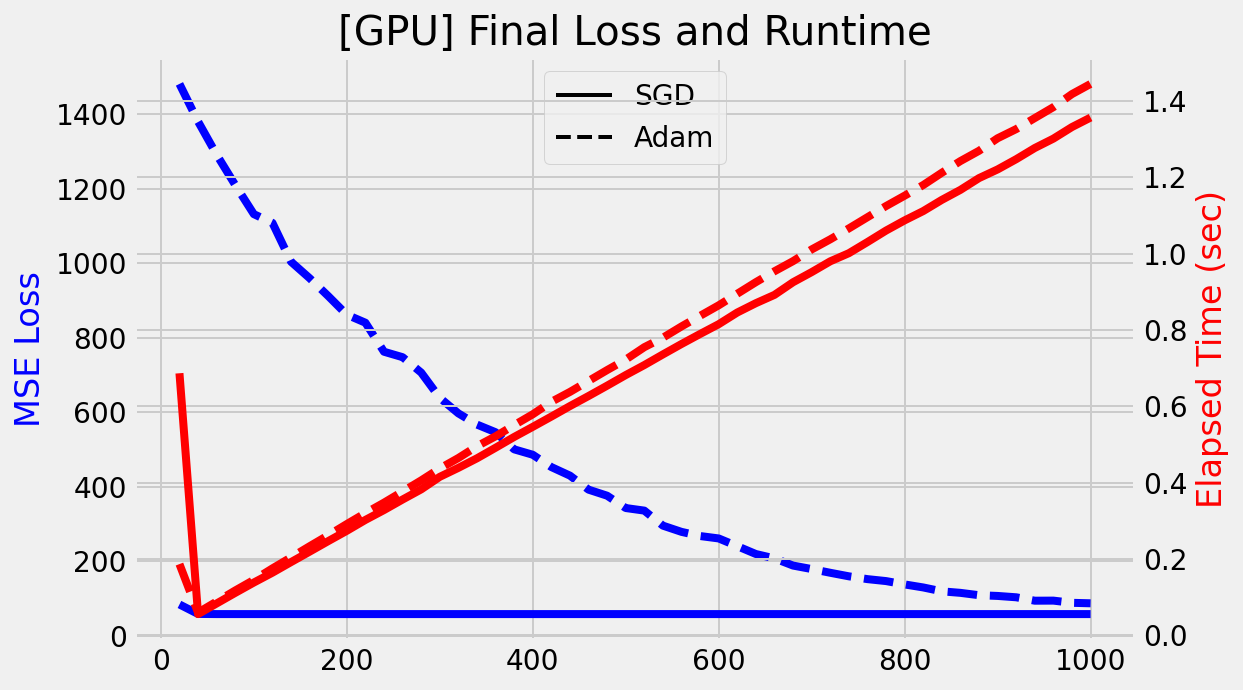
\includegraphics[width=\columnwidth]{figures/gpu_timing.png}
	\caption{GPU Final Training loss and Runtime vs Epochs}
	\label{fig:g}
\end{figure}

Out of curiosity I tried to see if I could demonstrate a significant GPU performance increase. To address the small dataset problem I created a $1,000,000$ point 50 feature data dataset with a trivial noise linear model. Figure~\ref{fig:g speedup} shows the final runtime for training it with the CPU and GPU. It can be seen that my GPU did improve performance by roughly a factor of 4. Meaning in the above experiment, had the dataset been larger the runtimes would've been improved.  

\begin{figure}[htpb]
	\centering
	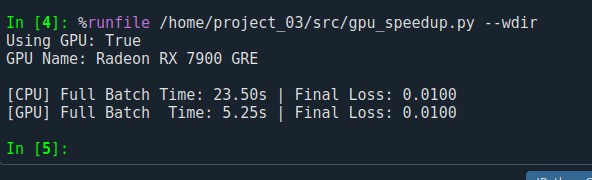
\includegraphics[width=\columnwidth]{figures/gpu_speedup.png}
	\caption{GPU Performance Increase}
	\label{fig:g speedup}
\end{figure}

